\documentclass[a4paper,9pt,twocolumn,twoside,]{pinp}

%% Some pieces required from the pandoc template
\providecommand{\tightlist}{%
  \setlength{\itemsep}{0pt}\setlength{\parskip}{0pt}}

% Use the lineno option to display guide line numbers if required.
% Note that the use of elements such as single-column equations
% may affect the guide line number alignment.

\usepackage[T1]{fontenc}
\usepackage[utf8]{inputenc}

% pinp change: the geometry package layout settings need to be set here, not in pinp.cls
\geometry{layoutsize={0.95588\paperwidth,0.98864\paperheight},%
  layouthoffset=0.02206\paperwidth, layoutvoffset=0.00568\paperheight}

\definecolor{pinpblue}{HTML}{185FAF}  % imagecolorpicker on blue for new R logo
\definecolor{pnasbluetext}{RGB}{101,0,0} %



\title{Executive summary}

\author[1]{Emlyn Bilbie}
\author[1]{Aiden Davies}
\author[1]{Joseph Isaacs}
\author[1]{Daniel Mechtersheimer}

  \affil[1]{T09oc\_early\_4, DATA2902, University of Sydney}

\setcounter{secnumdepth}{0}

% Please give the surname of the lead author for the running footer
\leadauthor{}

% Keywords are not mandatory, but authors are strongly encouraged to provide them. If provided, please include two to five keywords, separated by the pipe symbol, e.g:
 

\begin{abstract}
This report presents the findings of an investigation into predicting
the final Mathematics grades of secondary school students in Portugal by
performing multiple regression on the results of a survey given to
students of Portuguese and Mathematics. Two candidate models were
constructed through stepwise variable selection processes. The two
models performed simmilarly out-of-sample, so the smaller model was
selected, including earlier mathematics marks, family relationship
quality, age, and absences from class as predictors. However, the model
is prone to inaccuracy in predicting lower marks, and future
investigation could be conducted into an `early intervention' model that
does not include past grades.
\end{abstract}

\dates{This version was compiled on \today} 

\documentdate{20 November 2020}

% initially we use doi so keep for backwards compatibility
% new name is doi_footer
\doifooter{\url{https://github.sydney.edu.au/DMEC5133/T09oc_early_4}}

\pinpfootercontents{Executive summary}

\begin{document}

% Optional adjustment to line up main text (after abstract) of first page with line numbers, when using both lineno and twocolumn options.
% You should only change this length when you've finalised the article contents.
\verticaladjustment{-2pt}

\maketitle
\thispagestyle{firststyle}
\ifthenelse{\boolean{shortarticle}}{\ifthenelse{\boolean{singlecolumn}}{\abscontentformatted}{\abscontent}}{}

% If your first paragraph (i.e. with the \dropcap) contains a list environment (quote, quotation, theorem, definition, enumerate, itemize...), the line after the list may have some extra indentation. If this is the case, add \parshape=0 to the end of the list environment.


\hypertarget{introduction}{%
\section{Introduction}\label{introduction}}

Using a data set containing information about students in Portugal, and
their marks in Mathematics and Portuguese, this project aims to develop
a multiple rgression model to predict a student's Mathematics grade
based on the other variables in the data set. The model will incorporate
students' academic performance through the year, in order to provide
estimated final marks that could allow students to plan future studies
before receiving their final grade, or be used in the case of illness or
misadventure. In this report, we will detail the process that was used
to develop the model and discuss its effectiveness by examining model
stability, and its performance, both in- and out-of-sample.

\hypertarget{data-set}{%
\section{Data set}\label{data-set}}

The data set was retrieved from the \cite{uci}, and contains information
relating to students in Portugal, with each row representing a student
and each column representing some attribute about the student.

The data was collected for a study by the University of Minho in
2005--06 from two public schools, using school reports and
questionnaires \citep*{cortezsilva08}. Two data sets are included,
containing information on 395 students of Mathematics and 649 students
of Portuguese. Both contain 33 different attributes, with three being
grades for the respective subjects and 30 sourced from the questionnaire
given to students.

There are 382 students who are listed in both data sets, according to
its metadata. We expected that a student's performance in Portuguese
might be related to their performance in Mathematics, so for the
purposes of our analysis, we merged the two data sets, including only
these students.

However, there were several columns which were near-identical between
the two data sets, with only a few differing observations. Since these
were variables that would not sensibly differ based on the particular
subject described, we surmised that the differences may be due to the
survey for each subject being administered at slightly different points
in time. To avoid choosing between these near-identical columns in the
model selection, we filtered our dataset to only contain rows with the
same values for these columns, ending up with 320 rows and 38 columns.
The five subject-specific columns were the student's three grades
(\texttt{G1}, \texttt{G2}, \texttt{G3}), whether or not they paid for
extra classes in the subject (\texttt{paid}) and the number of absences
from the subject (\texttt{absences}). We also re-coded some numeric
variables that did not have linearly increasing categories as
categorical . These were the two parents' levels of educational
attainment (\texttt{Medu} and \texttt{Fedu}), as well as
\texttt{traveltime} and \texttt{studytime}.

\hypertarget{analysis}{%
\section{Analysis}\label{analysis}}

\hypertarget{assumption-checking}{%
\subsection{Assumption checking}\label{assumption-checking}}

In Fig. \ref{fig:resid-qq} it appears that the residuals of the model
are distributed randomly above and below zero, with the exception of a
problematic patch of much lower values. So, if we momentarily disregard
these points, the linear model does not appear to be unsuitable. There
is also no evidence of fanning or change in variability, so
homoskedasticity is fulfilled.

In the Q--Q plot, the straight line is closely followed for the majority
of the points, again with the exception of the lower values which
deviate quite notably. Despite this, there are enough values for the
central limit theorem to hold, so inferences based on the normality
assumption should be valid.

\begin{figure}[htbp]

{\centering 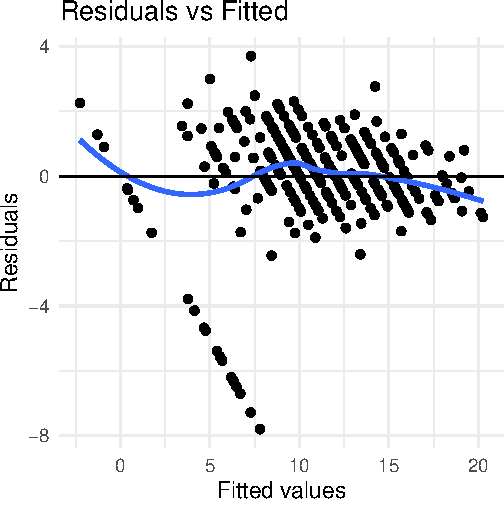
\includegraphics[width=0.45\linewidth]{Executive-summary_files/figure-latex/resid-qq-1} 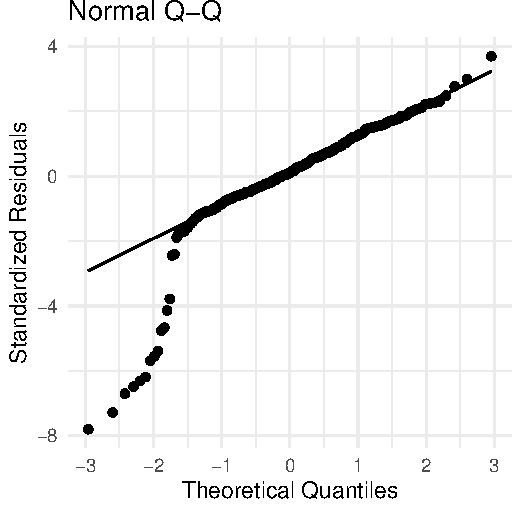
\includegraphics[width=0.45\linewidth]{Executive-summary_files/figure-latex/resid-qq-2} 

}

\caption{Residual and Q–Q plots for full model}\label{fig:resid-qq}
\end{figure}

Observing the pairs of plots in Fig. \ref{fig:pairs} (see Appendix), it
is clear that these troublesome lower points are resultant of a cluster
of students who received a mark of 0 for the final mathematics
assessment, despite doing well in other assessments. It is possible that
this is due to missing values, but since there are real-world
explanations for this (such as non-attempts or academic dishonesty), we
decided to retain the values. This does mean, however, that caution
should be taken when the model predicts smaller values (those below 7 or
8), keeping in mind that they may be inaccurate. However, for predicting
higher values, the assumptions are met.

Finally, we assume that all students' responses are independent of each
other, although we would need to confirm this with more information on
the students sampled.

\hypertarget{model-selection}{%
\subsection{Model selection}\label{model-selection}}

To construct a model for the final mathematics mark (\texttt{G3\_mat})
by means of multiple regression, we first carried out automated
backwards and forwards variable selection using the \texttt{step()}
function in R, which aims to minimise the model's Akaike information
criterion (AIC) value.

The automated backwards selection returned a model containing 12
variables. Using forward selection instead, the process returned a model
with 11 variables, of which 9 were common with the backwards model. Both
models had similarly high \(r^2\) values of approximately 0.86,
indicating that they were strong.

Further fine-tuning of both models was conducted manually. Adding
variables to either model did not produce any significant results.
Removing variables, however, proved to be more useful. By iteratively
assessing the result of removing a variable with R's \texttt{drop1()}
function, we managed to remove several insignificant variables from both
models. From our original `backwards' model, we ended up with only five
variables, while from our original `forwards' model, we ended up with
seven (see Table \ref{tab:new-models} in Appendix). The smaller models
allow accurate prediction (with similarly high \(r^2\) values), without
over-fitting by including too many predictor variables.

Figs. \ref{fig:resid-qq-5var} and \ref{fig:resid-qq-7var} (see Appendix)
show that the behaviour for our two new models is very similar to the
full model, so our assumptions still hold for higher values, with the
same caveat for lower-performing students.

\hypertarget{model-stability}{%
\subsection{Model stability}\label{model-stability}}

In order to analyse the stability of our models, we started with a model
stability plot for the 12 variables used in our original backwards model
(Fig. \ref{fig:model-stability}). There are no other models which appear
particularly dominant, with all groupings showing relatively equal
applicability.

\begin{figure}[htbp]

{\centering 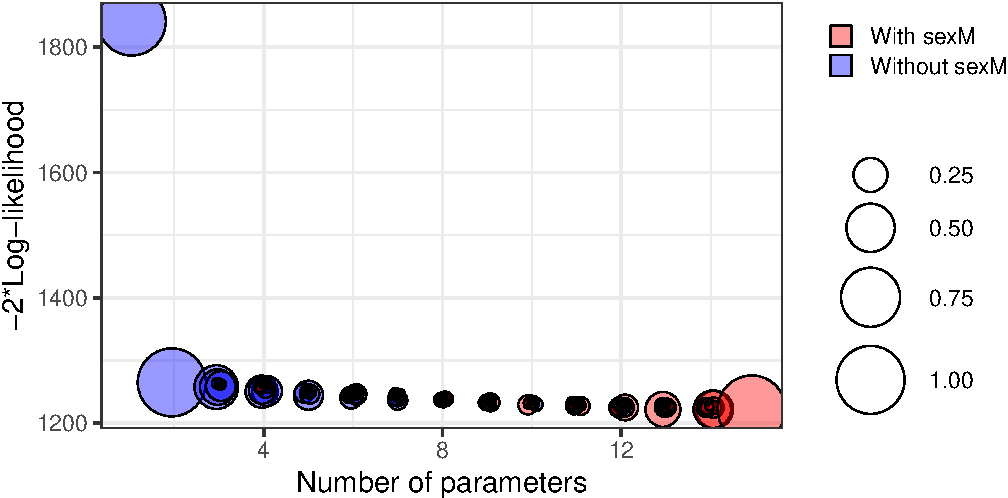
\includegraphics[width=0.85\linewidth]{Executive-summary_files/figure-latex/model-stability-1} 

}

\caption{Model stability plot}\label{fig:model-stability}
\end{figure}

A variable inclusion plot (Fig. \ref{fig:vip-plot}) clearly supports the
necessary inclusion of \texttt{G2\_mat} as a strong predictor variable.
The other predictors in our model are more varied, although there is
also evidence for their inclusion. So, we will retain both models found
with stepwise selection and assess their performance.

\begin{figure}[htbp]

{\centering 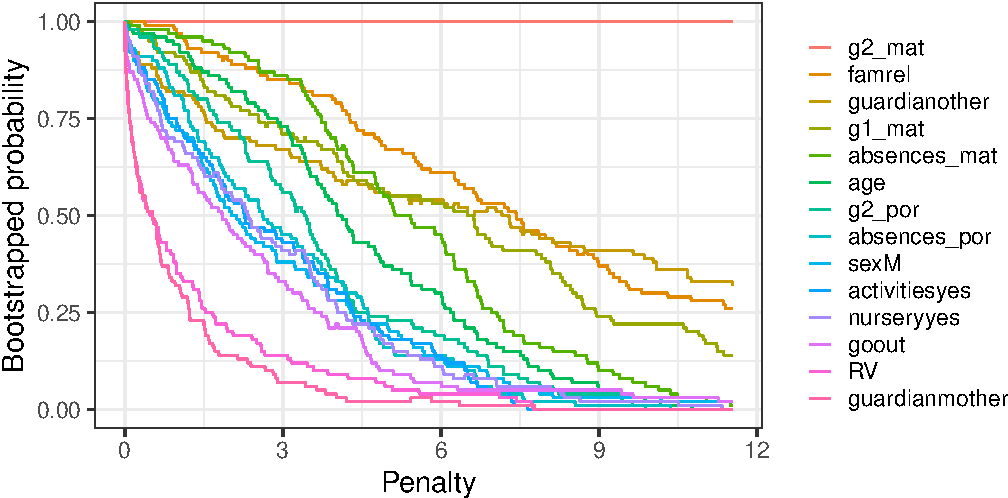
\includegraphics[width=0.85\linewidth]{Executive-summary_files/figure-latex/vip-plot-1} 

}

\caption{Variable inclusion plot}\label{fig:vip-plot}
\end{figure}

\hypertarget{results}{%
\section{Results}\label{results}}

\hypertarget{in-sample-assessment}{%
\subsection{In-sample assessment}\label{in-sample-assessment}}

Our larger and smaller models have very similar AIC values: 1252.96 and
1256.63 respectively. They also have similar \(r^2\) values: 0.849
compared to 0.846. While it is promising to see such strong in-sample
performance, the close results do not give us sufficient evidence to
select between the two models, or to make any conclusions as to the
models' actual effectiveness. Evaluation of the two models'
out-of-sample performance is needed to draw firmer conclusions.

\hypertarget{out-of-sample-assessment}{%
\subsection{Out-of-sample assessment}\label{out-of-sample-assessment}}

In order to assess out-of-sample performance, we conducted 10-fold
cross-validation estimation, using the caret package for R. For the
smaller model, we attained a root mean square error (RMSE) of 1.649 and
a mean absolute error (MAE) of 1.024. For the larger model, our RMSE was
1.651 and our MAE was 1.042.

As evidenced by the bootstrapped confidence intervals in Fig.
\ref{fig:out-sample}, these two errors are not significantly different,
meaning the two models performed very similarly overall. Since the more
complicated model does not provide any improvements to performance, it
makes sense to select the smaller, simpler model for easier computation.

\begin{figure}[htbp]

{\centering 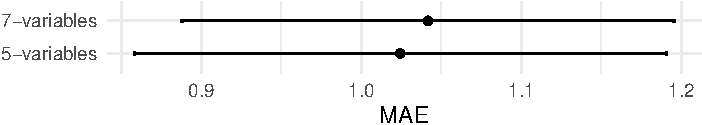
\includegraphics[width=0.85\linewidth]{Executive-summary_files/figure-latex/out-sample-1} 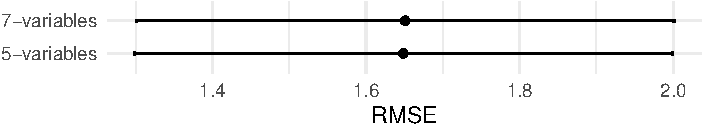
\includegraphics[width=0.85\linewidth]{Executive-summary_files/figure-latex/out-sample-2} 

}

\caption{Bootstrapped confidence intervals}\label{fig:out-sample}
\end{figure}

\hypertarget{final-model}{%
\subsection{Final model}\label{final-model}}

Since our selected model does not include any variables specific to
Portuguese, the model can be fitted against the original, larger
Mathematics data set. For this model, we get,

\[
\begin{aligned}
\operatorname{G3} &= -0.08 + 0.16(\operatorname{G1}) + 0.98(\operatorname{G2}) + 0.04(\operatorname{absences})\ + \\
&\quad 0.36(\operatorname{famrel}) - 0.2(\operatorname{age}) + \epsilon
\end{aligned}
\]

As expected, the final mathematics grade (\texttt{G3}) tends to increase
with the first and second period mathematics grades (\texttt{G1} and
\texttt{G2}). This relationship is stronger with \texttt{G2}. This is
reasonable since this is the mark that is closest in time to the final
mark, so students that do well in second period can be expected to do
similarly well in the final assessment. \texttt{G3} also increases with
better quality of family relationship (\texttt{famrel}), indicating that
satisfaction with the home environment and family support play
significant roles in success. Increases in \texttt{age} were associated
with a lower grade, possibly as a result of increasing difficulty in
later school grades. Further analysis of results across each grade would
be required to determine if this is the case. An unexpected result was
that more absences from class predicted higher marks. While one would
expect that missing class would negatively affect a student's
performance, it may also be possible that many absences from class
motivate students to study independently, positively impacting their
grades.

\hypertarget{discussion-and-conclusion}{%
\section{Discussion and conclusion}\label{discussion-and-conclusion}}

As expected, the strongest predictors were students' other marks, but
also their family relationship quality, age and absences. Our
out-of-sample performance is strong; however, our model may be prone to
inaccuracies for lower marks. Further information about the \texttt{G3}
marks recorded as 0 could help resolve this for future studies.

To apply this model across all schools in Portugal, a future study
should be conducted with data from a larger range of different schools,
located in different regions of the country. The geographical
similarities between the two schools in the data set may misrepresent
the relationship between certain variables when compared to students in
different regions. For example, if both schools surveyed were in
high-income areas then the model may be inaccurate in low-income areas.

A future study could also attempt to build a model without the
\texttt{G1} and \texttt{G2} marks as predictor variables, in order to
identify students who are at risk of under-performing at the start of
the school year. However, there are ethical issues that may be raised by
identifying these students based on personal characteristics such as sex
and family relationships.

\pagebreak

\nocite{*}

\bibliographystyle{apalike}
\bibliography{references}

\hypertarget{appendix}{%
\section{Appendix}\label{appendix}}

\begin{figure}[htbp]

{\centering 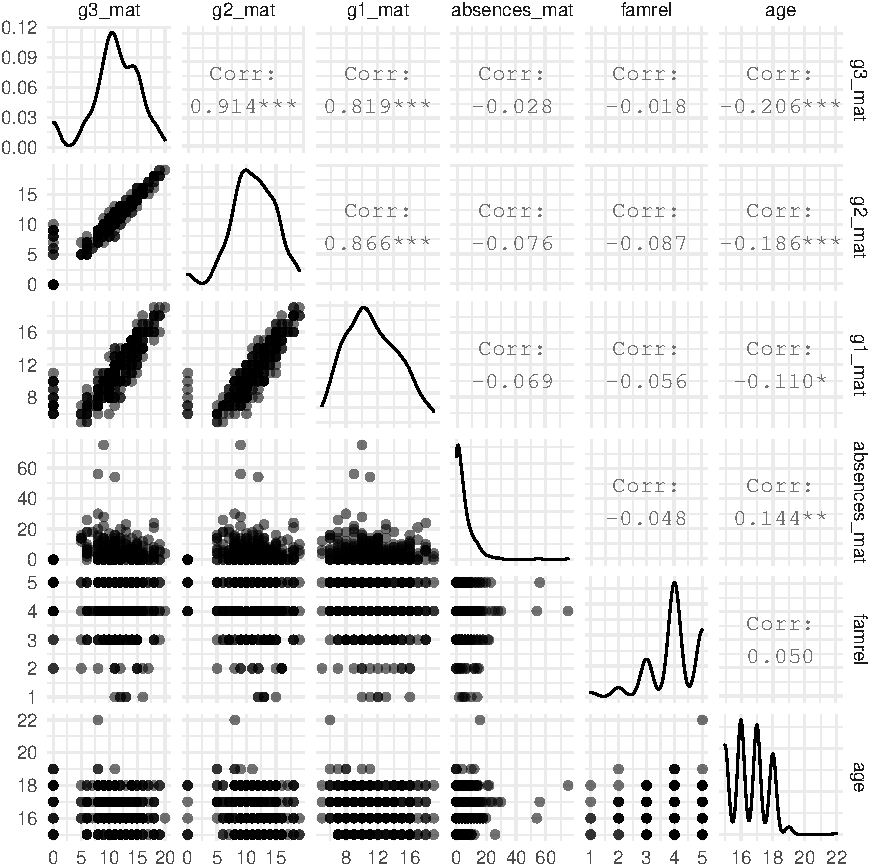
\includegraphics[width=1\linewidth]{Executive-summary_files/figure-latex/pairs-1} 

}

\caption{Pairs for seleted numeric variables}\label{fig:pairs}
\end{figure}

\begin{figure}[htbp]

{\centering 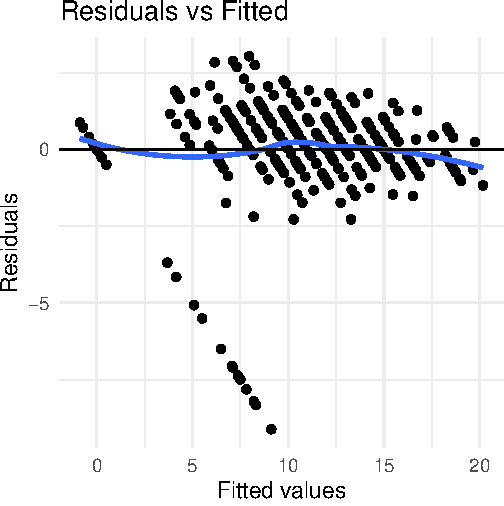
\includegraphics[width=0.45\linewidth]{Executive-summary_files/figure-latex/resid-qq-5var-1} 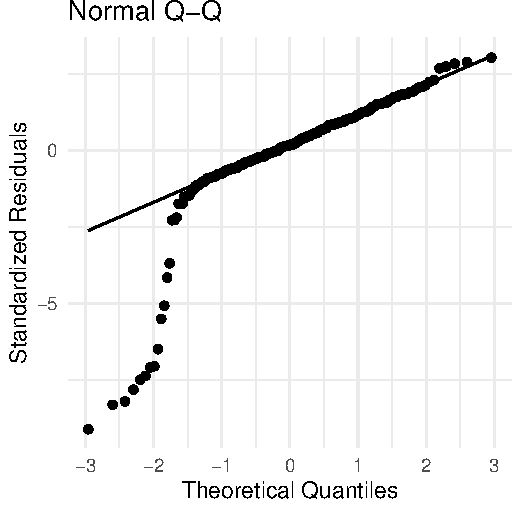
\includegraphics[width=0.45\linewidth]{Executive-summary_files/figure-latex/resid-qq-5var-2} 

}

\caption{Residual and Q-Q plots for 5-predictor model}\label{fig:resid-qq-5var}
\end{figure}

\begin{figure}[htbp]

{\centering 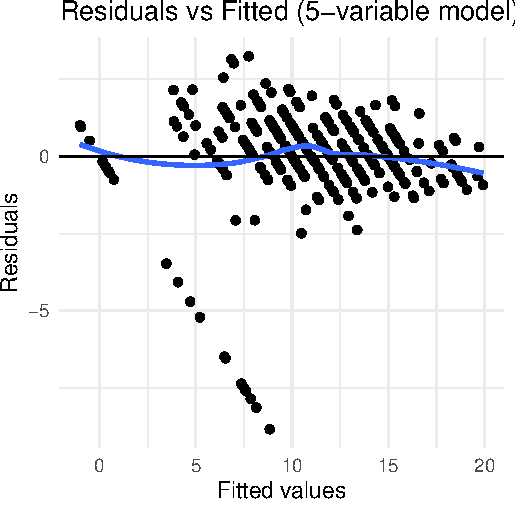
\includegraphics[width=0.45\linewidth]{Executive-summary_files/figure-latex/resid-qq-7var-1} 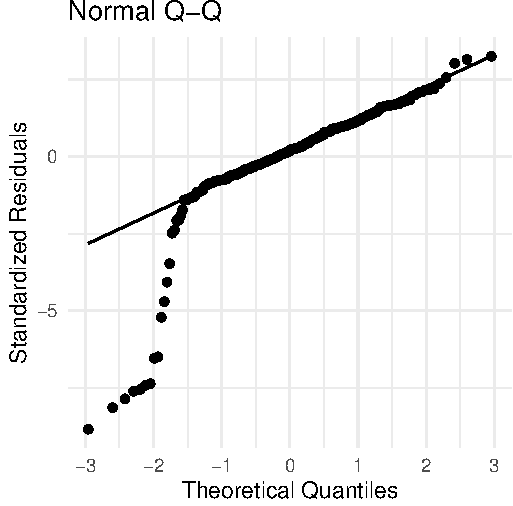
\includegraphics[width=0.45\linewidth]{Executive-summary_files/figure-latex/resid-qq-7var-2} 

}

\caption{Residual and Q-Q plots for 7-predictor model}\label{fig:resid-qq-7var}
\end{figure}

\begin{table}[!htbp] \centering 
  \caption{Updated models} 
  \label{tab:new-models} 
\tiny 
\begin{tabular}{@{\extracolsep{5pt}}lcc} 
\\[-1.8ex]\hline 
\hline \\[-1.8ex] 
 & \multicolumn{2}{c}{\textit{Dependent variable:}} \\ 
\cline{2-3} 
\\[-1.8ex] & \multicolumn{2}{c}{g3\_mat} \\ 
\\[-1.8ex] & (1) & (2)\\ 
\hline \\[-1.8ex] 
 g2\_mat & 0.933$^{***}$ & 0.952$^{***}$ \\ 
  & (0.053) & (0.053) \\ 
  & & \\ 
 famrel & 0.343$^{***}$ & 0.313$^{***}$ \\ 
  & (0.108) & (0.108) \\ 
  & & \\ 
 g1\_mat & 0.134$^{**}$ & 0.157$^{***}$ \\ 
  & (0.061) & (0.060) \\ 
  & & \\ 
 Walc & 0.177$^{**}$ &  \\ 
  & (0.079) &  \\ 
  & & \\ 
 age & $-$0.254$^{***}$ & $-$0.198$^{**}$ \\ 
  & (0.088) & (0.086) \\ 
  & & \\ 
 absences\_mat & 0.027$^{**}$ & 0.029$^{**}$ \\ 
  & (0.013) & (0.012) \\ 
  & & \\ 
 g2\_por & 0.100$^{**}$ &  \\ 
  & (0.051) &  \\ 
  & & \\ 
 Constant & 0.119 & 0.504 \\ 
  & (1.542) & (1.548) \\ 
  & & \\ 
\hline \\[-1.8ex] 
R$^{2}$ & 0.849 & 0.846 \\ 
Adjusted R$^{2}$ & 0.846 & 0.843 \\ 
Akaike Inf. Crit. & 1,252.957 & 1,256.634 \\ 
\hline 
\hline \\[-1.8ex] 
\textit{Note:}  & \multicolumn{2}{r}{$^{*}$p$<$0.1; $^{**}$p$<$0.05; $^{***}$p$<$0.01} \\ 
\end{tabular} 
\end{table}

%\showmatmethods

\pnasbreak 




\end{document}

